\documentclass[10pt]{article}
\pagenumbering{gobble}
\usepackage{graphicx}
\usepackage{hyperref}
\usepackage{listings}
\usepackage{xcolor}
\usepackage{textcomp}
\usepackage{color}


\definecolor{codegreen}{rgb}{0,0.6,0}
\definecolor{codegray}{rgb}{0.5,0.5,0.5}
\definecolor{codepurple}{HTML}{C42043}
\definecolor{backcolour}{HTML}{F2F2F2}
% \definecolor{bookColor}{cmyk}{0,0,0,0.90}  
% \color{bookColor}

\lstset{upquote=true}

\lstdefinestyle{mystyle}{
    backgroundcolor=\color{backcolour},   
    commentstyle=\color{codegreen},
    keywordstyle=\color{codepurple},
    numberstyle=\footnotesize\color{codegray},
    stringstyle=\color{codepurple},
    basicstyle=\footnotesize,
    breakatwhitespace=false,         
    breaklines=true,                 
    captionpos=b,                    
    keepspaces=true,                 
    numbers=left,                    
    numbersep=-10pt,                  
    showspaces=false,                
    showstringspaces=false,
    showtabs=false,      
}
\lstset{style=mystyle} 


\addtolength{\oddsidemargin}{-.875in}
	\addtolength{\evensidemargin}{-.875in}
	\addtolength{\textwidth}{1.75in}

	\addtolength{\topmargin}{-.875in}
	\addtolength{\textheight}{1.75in}
\renewcommand{\baselinestretch}{0.97}
\title{\textbf{Project 1: Music Recommender}}
% \author {\textbf{Sanket Hire (2016CS50402), Yash Malviya (2016CS50403), Vasudev Singh (2016MT60660)}}
\author{\textbf{Sanket Hire} \\ \textbf{2016CS50402} \and \textbf{Yash Malviya} \\ \textbf{2016CS50403} \and \textbf{Vasudev Singh} \\ \textbf{2016MT60660}} 

\date{Due date: March 2, 2020, 11:55pm IST}

\begin{document}

\maketitle

\section{Section 1}
This section provides brief description of our project.
\subsection{Motivation}
The main motive of this project is to provide a platform for music enthusiasts and listeners.This platform helps users in recommending songs of their taste and allow them to share their playlists with others.For automating the user music taste, we are developing the music recommendation system which recommends songs based on their listening history.User's listening history is being analysed on artist based features(artist name,  country,tags, listeners and scrobbles) and song based features(track, artist, danceability, energy, track key, loudness, mode, speechiness, acousticness,  instrumentalness,  liveness,  valence,  tempo,  duration,  time  signature,  chorus  hit,  track,sections and hit target). 


% \let\cleardoublepage\clearpage
% \newpage
\subsection{E-R Diagram}
\begin{center}
    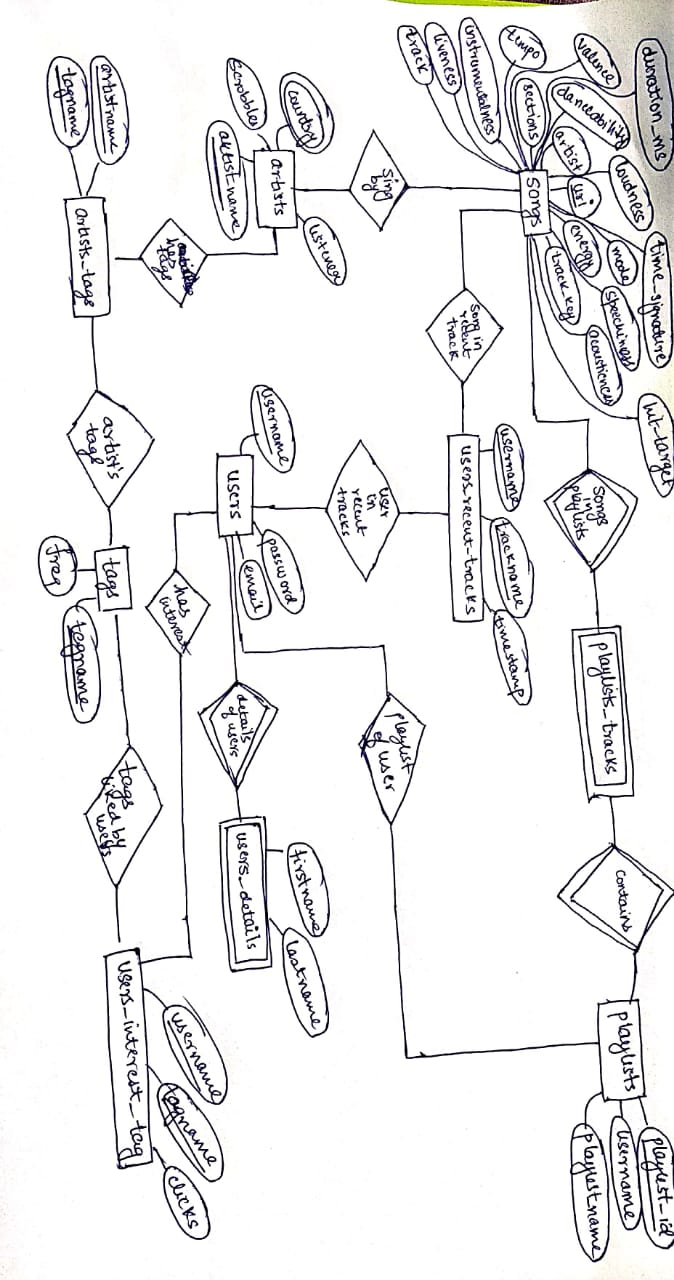
\includegraphics[width=\textwidth,height=\textheight,keepaspectratio]{ER_diagram.jpeg}
\end{center}

\subsection{List of Entities and Attributes}
\subsubsection{artists}
\label{sec:1.3.1}
\begin{table}[!ht]
    \centering
    \begin{tabular}{|l|l|}
         \hline
         \textbf{Attribute Name} & \textbf{Description} \\
         \hline
         artist\_name(\textbf{primary key}) & Name of the artist  \\
         \hline
         country(\textbf{Multi-valued attribute}) & Country to which artist belongs to  \\
         \hline
         listeners & Number of listeners on last.fm \\
         \hline
         scrobbles &  Number of scrobbles on last.fm\\
         \hline
    \end{tabular}
    \caption{artists}
    \label{tab:my_label1}
\end{table}

\begin{lstlisting}[language=SQL,
        deletekeywords={IDENTITY,INT},
        morekeywords={clustered},    
        framesep=10pt,
        framextopmargin=10pt]
    create table artists(
      artist_name text ,
      country text,
      listeners integer,
      scrobbles integer,
      primary key (artist_name)
    );
\end{lstlisting}

\subsubsection{songs}
\label{sec:1.3.2}
\begin{table}[!ht]
    \centering
    \begin{tabular}{|l|l|}
         \hline
         \textbf{Attribute Name} & \textbf{Description} \\
         \hline
         track & Name of the artist  \\
         \hline
         artist & Country to which artist belongs to  \\
         \hline
         uri(\textbf{primary key}) & The resource identifier for the track. \\
         \hline
         danceability &  \begin{tabular}[c]{@{}l@{}}Danceability describes how suitable a track is for dancing based on a combination of\\ musical elements \end{tabular}.\\
         \hline
         energy &  \begin{tabular}[c]{@{}l@{}}Energy is a measure from 0.0 to 1.0 and represents a perceptual measure of intensity\\ and activity.\end{tabular}.\\
         \hline
         track\_key &  \begin{tabular}[c]{@{}l@{}}The estimated overall key of the track. Integers map to pitches using standard Pitch\\ Class notation.\end{tabular}.\\
         \hline
         loudness &  The overall loudness of a track in decibels (dB).\\
         \hline
         mode &  \begin{tabular}[c]{@{}l@{}}Mode indicates the modality (major or minor) of a track, the type of scale from which\\ its melodic content is derived.\end{tabular}.\\
         \hline
         speechiness &  Speechiness detects the presence of spoken words in a track.\\
         \hline
         acousticness &  A confidence measure from 0.0 to 1.0 of whether the track is acoustic.\\
         \hline
         instrumentalness &  Predicts whether a track contains no vocals.\\
         \hline
         liveness &  Detects the presence of an audience in the recording.\\
         \hline
         valence &  A measure from 0.0 to 1.0 describing the musical positiveness conveyed by a track.\\
         \hline
         tempo &  The overall estimated tempo of a track in beats per minute (BPM).\\
         \hline
         duration\_ms &  The duration of the track in milliseconds.\\
         \hline
         time\_signature &  \begin{tabular}[c]{@{}l@{}}The time signature (meter) is a notational convention to specify how many beats are in each\\ bar (or measure).\end{tabular}.\\
         \hline
         chorus hit &  This the the author's best estimate of when the chorus would start for the track.\\
         \hline
         sections &  The number of sections the particular track has.\\
         \hline
         hit\_target &  \begin{tabular}[c]{@{}l@{}}It can be either '0' or '1'. '1' implies that this song has featured in the weekly list (Issued by\\ Billboards) of Hot-100 tracks in that decade at least once and is therefore a 'hit'. '0' Implies\\ that the track is a 'flop'.\end{tabular}.\\
         \hline
    \end{tabular}
    \caption{songs}
    \label{tab:my_label2}
\end{table}

\begin{lstlisting}[language=SQL,
        deletekeywords={IDENTITY,INT},
        morekeywords={clustered},    
        framesep=10pt,
        framextopmargin=10pt]
    create table songs(
      track text,
      artist text,
      uri varchar(36),
      danceability decimal,
      energy decimal,
      track_key integer,
      loudness decimal,
      mode decimal,
      speechiness decimal,
      acousticness decimal,
      instrumentalness decimal,
      liveness decimal,
      valence decimal,
      tempo decimal,
      duration_ms integer,
      time_signature integer,
      chorus_hit decimal,
      sections integer,
      hit_target integer,
      primary key (uri),
      foreign key (artist) references artists(artist_name) on delete cascade on update cascade
    );
\end{lstlisting}

\subsubsection{tags}
\label{sec:1.3.3}
\begin{table}[!ht]
    \centering
    \begin{tabular}{|l|l|}
         \hline
         \textbf{Attribute Name} & \textbf{Description} \\
         \hline
         tag\_name(\textbf{primary key}) & Tag of the artist  \\
         \hline
         freq &  Frequency of the tags\\
         \hline
    \end{tabular}
    \caption{tags}
    \label{tab:my_label3}
\end{table}

\begin{lstlisting}[language=SQL,
        deletekeywords={IDENTITY,INT},
        morekeywords={clustered},    
        framesep=10pt,
        framextopmargin=10pt]
    create table tags(
      tag_name text unique,
      freq integer,
      primary key(tag_name)
    );
\end{lstlisting}

\subsubsection{artist\_tags}
\label{sec:1.3.4}
\begin{table}[!ht]
    \centering
    \begin{tabular}{|l|l|}
         \hline
         \textbf{Attribute Name} & \textbf{Description} \\
         \hline
         artist\_name & Name of the artist  \\
         \hline
         tag\_name &  Tag of the artist\\
         \hline
    \end{tabular}
    \caption{artist\_tags}
    \label{tab:my_label4}
\end{table}

\begin{lstlisting}[language=SQL,
        deletekeywords={IDENTITY,INT},
        morekeywords={clustered},    
        framesep=10pt,
        framextopmargin=10pt]

    create table artist_tags(
      artist_name text,
      tag_name text,
      primary key (artist_name, tag_name), 
      foreign key (artist_name) references artists(artist_name) on delete cascade on update cascade,
      foreign key (tag_name) references tags(tag_name) on delete cascade on update cascade
    );

\end{lstlisting}

\subsubsection{users}
\begin{table}[!ht]
    \centering
    \begin{tabular}{|l|l|}
         \hline
         \textbf{Attribute Name} & \textbf{Description} \\
         \hline
         username & Username of User  \\
         \hline
         email &  Email of User\\
         \hline
         passwd &  Password of User\\
         \hline
    \end{tabular}
    \caption{users}
    \label{tab:my_label5}
\end{table}

\begin{lstlisting}[language=SQL,
        deletekeywords={IDENTITY,INT},
        morekeywords={clustered},    
        framesep=10pt,
        framextopmargin=10pt]
    create table users(
      username text,
      email text unique,
      passwd text,
      primary key (username)
    );
\end{lstlisting}

\subsubsection{user\_details}
\begin{table}[!ht]
    \centering
    \begin{tabular}{|l|l|}
         \hline
         \textbf{Attribute Name} & \textbf{Description} \\
         \hline
         username & Username of User  \\
         \hline
         email &  Email of User\\
         \hline
         passwd &  Password of User\\
         \hline
    \end{tabular}
    \caption{user\_details}
    \label{tab:my_label6}
\end{table}

\begin{lstlisting}[language=SQL,
        deletekeywords={IDENTITY,INT},
        morekeywords={clustered},    
        framesep=10pt,
        framextopmargin=10pt]
    create table user_details(
      username text ,
      first_name varchar(32),
      last_name varchar(32),
      primary key (username),
      foreign key (username) references users(username) on delete cascade on update cascade
    );
\end{lstlisting}

\subsubsection{playlists}
\begin{table}[!ht]
    \centering
    \begin{tabular}{|l|l|}
         \hline
         \textbf{Attribute Name} & \textbf{Description} \\
         \hline
         playlist\_id(\textbf{primary key}) & Playlist Id  \\
         \hline
         username &  Username of User\\
         \hline
         playlist\_name &  Name Of Playlist\\
         \hline
    \end{tabular}
    \caption{playlists}
    \label{tab:my_label7}
\end{table}

\begin{lstlisting}[language=SQL,
        deletekeywords={IDENTITY,INT},
        morekeywords={clustered},    
        framesep=10pt,
        framextopmargin=10pt]
    create table playlists(
      playlist_id serial,
      username text,
      playlist_name text,
      primary key (playlist_id),
      foreign key (username) references users(username) on delete cascade on update cascade
    );
\end{lstlisting}

\subsubsection{playlist\_tracks}
\begin{table}[!ht]
    \centering
    \begin{tabular}{|l|l|}
         \hline
         \textbf{Attribute Name} & \textbf{Description} \\
         \hline
         playlist\_id & Playlist Id  \\
         \hline
         track\_uri &  link for the track\\
         \hline
    \end{tabular}
    \caption{playlist\_tracks}
    \label{tab:my_label8}
\end{table}

\begin{lstlisting}[language=SQL,
        deletekeywords={IDENTITY,INT},
        morekeywords={clustered},    
        framesep=10pt,
        framextopmargin=10pt]
    create table playlist_tracks(
      playlist_id integer,
      track_uri varchar(36),
      primary key (playlist_id, track_uri),
      foreign key (playlist_id) references playlists(playlist_id) on delete cascade on update cascade,
      foreign key (track_uri) references songs(uri) on delete cascade on update cascade
    );
\end{lstlisting}

\subsubsection{user\_interest\_tags}
\begin{table}[!ht]
    \centering
    \begin{tabular}{|l|l|}
         \hline
         \textbf{Attribute Name} & \textbf{Description} \\
         \hline
         username & Username of user\\
         \hline
         tag\_name &  Tag of the artist\\
         \hline
         clicks &  Number of times the tag got queried\\
         \hline         
    \end{tabular}
    \caption{user\_interest\_tags}
    \label{tab:my_label9}
\end{table}

\begin{lstlisting}[language=SQL,
        deletekeywords={IDENTITY,INT},
        morekeywords={clustered},    
        framesep=10pt,
        framextopmargin=10pt]
    create table user_interest_tags(
      username text,
      tag_name text,
      clicks integer,
      primary key (username, tag_name),
      foreign key (username) references users(username) on delete cascade on update cascade,
      foreign key (tag_name) references tags(tag_name) on delete cascade on update cascade
    );
\end{lstlisting}

\subsubsection{user\_recent\_tracks}
\begin{table}[!ht]
    \centering
    \begin{tabular}{|l|l|}
         \hline
         \textbf{Attribute Name} & \textbf{Description} \\
         \hline
         username & Username of user\\
         \hline
         track\_uri &  link of the track\\
         \hline
         time\_stamp &  timestamp at which the song got requested to play\\
         \hline         
    \end{tabular}
    \caption{user\_recent\_tracks}
    \label{tab:my_label10}
\end{table}

\begin{lstlisting}[language=SQL,
        deletekeywords={IDENTITY,INT},
        morekeywords={clustered},    
        framesep=10pt,
        framextopmargin=10pt]
    create table user_recent_tracks(
      username text,
      track_uri varchar(36),
      time_stamp timestamp,
      primary key (username, track_uri),
      foreign key (username) references users(username) on delete cascade on update cascade,
      foreign key (track_uri) references songs(uri) on delete cascade on update cascade
    );
\end{lstlisting}

\section{Section 2}
\subsection{Sources of our data}
\label{sec:2.1}
\begin{itemize}
    \item Music artists popularity:  \href{https://www.kaggle.com/pieca111/music-artists-popularity}{\textbf{https://www.kaggle.com/pieca111/music-artists-popularity}} 
    \item The Spotify Hit Predictor Dataset (1960-2019): \href{https://www.kaggle.com/theoverman/the-spotify-hit-predictor-dataset}{\textbf{https://www.kaggle.com/theoverman/the-spotify-hit-predictor-dataset}}
\end{itemize}

\subsection{How we downloaded it}
We downloaded the "READYMADE" datasets from the links given in sources section\textbf{(\autoref{sec:2.1})}. 

\subsection{Cleanup Steps}
% \begin{enumerate}
\begin{itemize}
    \item We first downloaded the datasets as per \textbf{(\autoref{sec:2.1})}
    \begin{itemize}
        \item \textbf{Music artists popularity:} Artists dataset comprising the attributes -  artist\_name, country, tags, listeners, and scrobbles
        \begin{itemize}
            \item \textbf{"artists\_raw" table}
        \end{itemize}
    \item \textbf{The Spotify Hit Predictor Dataset (1960-2019):} Songs dataset comprising the attributes for tracks such as track, artist, danceability,  energy, track key,  loudness,  mode,  speechiness,  acousticness,  instrumentalness, liveness,  valence,  tempo,  duration, time signature, chorus hit, track sections, and hit target.
    \begin{itemize}
            \item \textbf{dataset-of-00s.csv}
            \item \textbf{dataset-of-10s.csv}
            \item \textbf{dataset-of-60s.csv}
            \item \textbf{dataset-of-70s.csv}
            \item \textbf{dataset-of-80s.csv}
            \item \textbf{dataset-of-90s.csv}
    \end{itemize}
    We compiled the above csv files of songs dataset in one table \textbf{"songs\_raw" table}
        
        \item \textbf{artists table} 
        \begin{itemize}
            \item Then we extracted the column attributes of \textbf{"artists\_raw" table} - artist\_name, country, listeners, and scrobbles. 
            \item and created \textbf{"artists" table} as shown in \textbf{(\autoref{sec:1.3.1})}. 
            \item With artist\_name as a distinct attribute. 
            \item Additionally, keeping only those artists which have sung the songs as per \textbf{"songs" table} by using \textbf{join}.    
        \end{itemize}
        
        \item \textbf{songs table}
        \begin{itemize}
            \item We extracted all the column attributes of \textbf{"songs\_raw" table}. 
            \item Keeping those rows in which songs have a artist existing in \textbf{"artists\_raw" table} by using \textbf{join}.
            \item Stored the table in \textbf{"songs" table} as shown in \textbf{(\autoref{sec:1.3.2})}.
        \end{itemize}
        
        \item \textbf{tags table}
        \begin{itemize}
            \item This table contains (tag\_name $\,\to\,$ freq(tag\_frequency)).
            \item tag\_name is distinct attribute extracted from \textbf{"artists\_tags" table's} tags attribute column. 
            \item freq(tag\_frequency) is the frequency of each tag present in \textbf{"artists\_tags" table's} tags attribute column. 
            \item Stored the table in \textbf{"tags" table} as shown in \textbf{(\autoref{sec:1.3.3})}.
        \end{itemize}
        
        \item \textbf{artists\_tags table}
        \begin{itemize}
            \item Further extracted the column attributes of \textbf{"artists\_raw" table} - artist\_name and tags (keeping artist\_name distinct across the rows). 
            \item Here tags were multi-valued for each artist. 
            \item So we created 1NF (artist\_name $\,\to\,$ tags) table and stored the table as \textbf{"artist\_tags" table} as shown in \textbf{(\autoref{sec:1.3.4})}.    
        \end{itemize}
        
        \item The tables below are for user queries which can be updated as per the user's input
        \\(Here, cleaning steps are not required at the database making stage):
        \begin{itemize}
            \item users
            \item user\_details
            \item playlists
            \item playlist\_tracks
            \item user\_interest\_tags
            \item user\_recent\_tracks
        \end{itemize}
        
    \end{itemize}

\end{itemize}
        
% \end{enumerate}
\newpage
\subsection{Statistics}
\begin{table}[!ht]
    \centering
    \begin{tabular}{|l|l|l|l|l|}
         \hline
         \textbf{Table} & \textbf{No. of Tuples} & \textbf{Time to Load} & \textbf{Raw Dataset Size} & \textbf{Raw Dataset Size (Clean)}\\
         \hline
         artists\_raw & 1466083 & 3675.145 ms & 201.1 MB & - \\
         \hline
         songs\_raw & 41106 & 264.162 ms & 7728 kB & - \\
         \hline
         artists & 7559 & * & - & 1024 kB \\
         \hline
         songs & 32025 & * & - & 7872 kB \\
         \hline
         tags & 7229 & * & - & 616 kB \\
         \hline
         artist\_tags & 221212 & * & - & 21 MB \\
         \hline
         users & 1 & - & - & 24 kB \\
         \hline
         user\_details & 1 & - & - & 16 kB \\
         \hline
         playlists & 2 & - & - & 16 kB \\
         \hline
         playlist\_tracks & 40 & - & - & 8192 bytes \\
         \hline
         user\_interest\_tags & 786 & - & - & 16 kB \\
         \hline
         user\_recent\_tracks & 10 & - & - & 16 kB \\
         \hline
    \end{tabular}
    \caption{Statistics}
    \label{tab:my_label11}
\end{table}

\textbf{[*]} These tables are not loaded from the csv but are the derived from the postgresql tables artist\_raw and songs\_raw that's why we have not written the time to load from them. Only query time can be deduced for these tables.

\section{Section 3}
\subsection{User's view of the system}
\begin{itemize}
    \item Login
    \begin{itemize}
        \item User is authenticated using a form to fill their username and password at the start
    \end{itemize}
    \item SignUp
    \begin{itemize}
        \item Interface for new users to create an account
        \item User is required to fill certain details such as his/her first name, last name along with username, email and password.
    \end{itemize}
    \item Update User's details
    \begin{itemize}
        \item User details has email, First Name, Last Name
        \item There is an interface to update this
    \end{itemize}
    \item Create Playlist
    \begin{itemize}
        \item This gives users option to save songs as a list and name the list
    \end{itemize}
    \item Add song to playlist
    \begin{itemize}
        \item Adding the a song the list described above
    \end{itemize}
    \item Play / Mark song
    \begin{itemize}
        \item This is most basic option of the application, where user can a song info or play it
    \end{itemize}
    \item Search
    \begin{itemize}
        \item A box to write in to search for songs and artists and various filtering and sorting options for the output
    \end{itemize}
    \item Recommendation
    \begin{itemize}
        \item from the perspective of the user, they will be able to see songs similar to the songs they hear the most
    \end{itemize}
\end{itemize}

\subsection{System view}
\begin{itemize}
     \item Signup
    \begin{itemize}
        \item A new entry is being inserted into users table whenever a user signs up
        \item Insert user data in user related entities such as users, user\_details.
    \end{itemize}
    \item Update User's Details
    \begin{itemize}
        \item User privilege to update user\_details attributes like user's username, first name and last name if requested. 
    \end{itemize}
    \item Create Playlist
    \begin{itemize}
        \item A new entry is being added into the playlists table signifying the playlist id and the owner of that playlist.
    \end{itemize}
     \item Add song to playlist
     \begin{itemize}
         \item A new entry is being inserted into the playlist\_tracks signifying the song name added to which playlist\_id.
     \end{itemize}
     \item Search 
     \begin{itemize}
        \item System administrator has a privilege to do search queries using "WHERE" clause for getting required tuples of attributes for a given set of conditions.
         \item Example: Return the list of songs sung by an artist. 
         \begin{lstlisting}[language=SQL,
                deletekeywords={IDENTITY,INT},
                morekeywords={clustered},    
                framesep=10pt,
                framextopmargin=10pt]
    select track from songs where artist = 'Drake';
            \end{lstlisting}
     \end{itemize}
    \item Recommendation
    \begin{itemize}
        \item Music is recommended using various information collected from the user as they operate the website 
        \item Type 1: User interest tags entire history
        \begin{itemize}
            \item Artist with most matching tags with user interest tags are selected. The songs these artist created are recommended to them. Note that this is based on which tags they are interested in not how much they are interested in it.
            \item Query: 
            \begin{lstlisting}[language=SQL,
                deletekeywords={IDENTITY,INT},
                morekeywords={clustered},    
                framesep=10pt,
                framextopmargin=10pt]
        select 
    	*
    from
    	(select
    	*
    	from (
    		select
    		arts.artist_name,
    		count(arts.artist_name)
    		from (
    			select
    			artist_name
    			from (
    				select
    				tag_name
    				from user_interest_tags
    				where
    				username = 'yash98'
    			) as in_tr,
    			artist_tags
    			where
    			artist_tags.tag_name = in_tr.tag_name
    		) as arts
    		group by
    		arts.artist_name
    	) as arts_count
    	order by
    	count desc) as arts_desc,
    	songs
    where arts_desc.artist_name = songs.artist;
            \end{lstlisting}
        \item time: 4 sec 754 msec
        \end{itemize}
        \item Type 2: User interest tags clicks based
        \begin{itemize}
            \item Clicks denote how much user is interested in a particular tag. The query for this type of recommendation calculates clicks for the tags an artist has. Based on this artists priority for being recommended is calculated.
            \item Query: 
            \begin{lstlisting}[language=SQL,
                deletekeywords={IDENTITY,INT},
                morekeywords={clustered},    
                framesep=10pt,
                framextopmargin=10pt]
    select 
    	*
    from
    	(select
    	*
    	from (
    		select
    		arts.artist_name,
    		sum(arts.clicks)
    		from (
    			select
    			artist_name, in_tr.tag_name, clicks
    			from (
    				select
    				tag_name, clicks
    				from user_interest_tags
    				where
    				username = 'yash98'
    			) as in_tr,
    			artist_tags
    			where
    			artist_tags.tag_name = in_tr.tag_name
    		) as arts
    		group by
    		arts.artist_name) as arts_sum
    	order by
    	sum desc) as arts_desc,
    	songs
    where arts_desc.artist_name = songs.artist;
    \end{lstlisting}
    \item time: 4 sec 719 msec
        \end{itemize}
    \item Type 3: Recent Tracks based
    \begin{itemize}
        \item This extract tags from artist of a song then proceed to rank other artists the same way as in type 1.
    \end{itemize}
    \end{itemize}
\end{itemize}

\subsubsection{Special functionality}
\begin{itemize}
    \item \textbf{Indexing}
    \begin{enumerate}
        \item \textbf{artist\_country\_index}
        \begin{lstlisting}[language=SQL,
                deletekeywords={IDENTITY,INT},
                morekeywords={clustered},    
                framesep=10pt,
                framextopmargin=10pt]
    create index artist_country_index on artists using brin(country);
            \end{lstlisting}
        \begin{enumerate}
            \textbf{Query}:
            \begin{lstlisting}[language=SQL,
                deletekeywords={IDENTITY,INT},
                morekeywords={clustered},    
                framesep=10pt,
                framextopmargin=10pt]
    select artist_name from artists where country = 'India';
            \end{lstlisting}
            \item index activate $\,\to\,$ \textbf{Time: 2.421 ms}
            \item index deactivate $\,\to\,$ \textbf{Time: 2.798 ms}
        \end{enumerate}
        \item \textbf{artist\_tag\_index}
        \begin{lstlisting}[language=SQL,
                deletekeywords={IDENTITY,INT},
                morekeywords={clustered},    
                framesep=10pt,
                framextopmargin=10pt]
    create index artist_tag_index on artist_tags using brin(tag_name);
            \end{lstlisting}
        \begin{enumerate}
            \textbf{Query}:
            \begin{lstlisting}[language=SQL,
                deletekeywords={IDENTITY,INT},
                morekeywords={clustered},    
                framesep=10pt,
                framextopmargin=10pt]
    select * from artist_tags where tag_name = 'rock';
            \end{lstlisting}
            \item index activate $\,\to\,$ \textbf{Time: 45.183 ms}
            \item index deactivate $\,\to\,$ \textbf{Time: 46.649 ms}
            
        \end{enumerate}
        \item \textbf{track\_artist\_index}
        \begin{lstlisting}[language=SQL,
                deletekeywords={IDENTITY,INT},
                morekeywords={clustered},    
                framesep=10pt,
                framextopmargin=10pt]
    create index track_artist_index on songs using brin(artist);
            \end{lstlisting}
        \begin{enumerate}
            \item \textbf{Query 1}:
            \begin{lstlisting}[language=SQL,
                deletekeywords={IDENTITY,INT},
                morekeywords={clustered},    
                framesep=10pt,
                framextopmargin=10pt]
    select track, artist from songs where artist = 'AC/DC';
            \end{lstlisting}
            \textbf{(6 Rows)}
            \begin{enumerate}
                \item index activate $\,\to\,$ \textbf{Time: 7.187 ms}
                \item index deactivate $\,\to\,$ \textbf{Time: 6.806 ms}
                
            \end{enumerate}
            \item \textbf{Query 2}:
            \begin{lstlisting}[language=SQL,
                deletekeywords={IDENTITY,INT},
                morekeywords={clustered},    
                framesep=10pt,
                framextopmargin=10pt]
    select track, artist from songs where artist = 'Taylor Swift';
            \end{lstlisting}
            \textbf{(49 Rows)}
            \begin{enumerate}
                \item index activate $\,\to\,$ \textbf{Time: 6.251 ms}
                \item index deactivate $\,\to\,$ \textbf{Time: 6.768 ms}
                
            \end{enumerate}
        \end{enumerate}
    \end{enumerate}
    
     \item \textbf{Trigger}
     \begin{itemize}
        \item It was used for two purposes
        \begin{itemize}
            \item Maintain the upper limit of stored recent track for each user. This maintains fixed number of songs that the user listened last i.e. it maintains first in first out
            \item Update tags user is interested as they listen to / mark a track. Increment clicks for a tag that user showed interest for.
        \end{itemize}
         \item \textbf{Query:}
         \begin{lstlisting}[language=SQL,
                deletekeywords={IDENTITY,INT},
                morekeywords={clustered},    
                framesep=10pt,
                framextopmargin=10pt]
    create or replace function trigger_add_recent_track() returns trigger as $body$ begin if (
      select
        count(*)
      from user_recent_tracks
      where
        user_recent_tracks.username = new.username
    ) >= 20 then begin
    delete from user_recent_tracks
    where
      new.username = user_recent_tracks.username
      and user_recent_tracks.time_stamp = (
        select
          min(time_stamp)
        from user_recent_tracks
        where
          new.username = user_recent_tracks.username
      );
    end;
    end if;
    update user_interest_tags
    set
      clicks = clicks + 1
    where
      user_interest_tags.tag_name in (
        (
          select
            user_interest_tags.tag_name
          where
            user_interest_tags.username = new.username
        )
        intersect
          (
            select
              artist_tags.tag_name
            from artist_tags
            where
              artist_tags.artist_name = (
                select
                  artist
                from songs
                where
                  songs.uri = new.track_uri
              )
          )
      );
    insert into user_interest_tags
    select
      new.username,
      q1.tag_name,
      1
    from (
        (
          select
            artist_tags.tag_name
          from artist_tags
          where
            artist_tags.artist_name = (
              select
                artist
              from songs
              where
                songs.uri = new.track_uri
            )
        )
        except
          (
            select
              user_interest_tags.tag_name
            from user_interest_tags
            where
              user_interest_tags.username = new.username
          )
      ) as q1;
    return new;
    end $body$ language plpgsql;
    
    
    create trigger add_recent_track before
    insert on user_recent_tracks for each row execute procedure trigger_add_recent_track();

            \end{lstlisting}
     \end{itemize}
     
\end{itemize}

\subsection{Timings}

Timings have been stated along with queries

\end{document}

